\documentclass[10pt,a4paper]{article}
%]{report}

\usepackage[a4paper, top=2cm, bottom=2.5cm, left=3cm, right=3cm]{geometry}
%\usepackage[
%    vmarginratio=2:2.5, %Verh�ltnis der oben/unten Seitenr�nder zur automatischen Berechnung
%    paper=a4paper,
%    lmargin=3cm, % mittlerer Rand
%    rmargin=3cm, % �u�erer Rand
%    marginparwidth=2.3cm, % Breite des Marginpars
%    includehead, % Kopfzeile in Berechnung einbeziehen
%    includemp % Marginpar in die Berechnung mit einbeziehen
%]{geometry}
%\setlength\marginparwidth{2.3cm} %Die wird sp�ter zum Rechnen gebraucht, wird aber durch die Angabe im geometry package nicht automatisch richtig gesetzt.


%============================================================
% Pakete
%============================================================

\usepackage[english, ngerman]{babel}    % mehrsprachiger Textsatz
% babel: letzte Sprache in Optionen zeigt die Sprache des Dokumentes
% und kann durch den Befehl \selectlanguage{} geaendert werden
% Passen Sie die Optionen des babel-Paketes nach Bedarf an!
\usepackage[utf8]{inputenc}       % Eingabekodierung Parameter latin1 darf ge�ndert werden
\usepackage[T1]{fontenc}                % Schriftenkodierung
\usepackage{graphicx}                       % zum Einbinden von Grafiken
\usepackage{lmodern}                        % Ersatz fuer Computer Modern-Schriften
                                                                % zum besseren Aussehen am Bildschirm
\usepackage{epstopdf}		% Grafiken einbinden
\usepackage{caption}		%Grafiken beschriften
%\usepackage{verbatimfiles}	% Ganze Dateien als Verbatim einbinden
% \usepackage{programs}	% Ganze Dateien als Verbatim einbinden
\usepackage{verbatim}		% Mehrzeilige Kommentare
\usepackage{multicol}		% Mehrere Spalten
\usepackage{hyphsubst}		% Silbentrennung
\usepackage{xcolor,soul}
\usepackage{float}				%Sachen an der richtigen Stelle ausgeben
\restylefloat{figure}				%Abbildungen an der richtigen Stelle ausgeben
\restylefloat{table}				%Tabellen an der richtigen Stelle ausgeben
\usepackage{array}				%f�r Tabellen
\newcolumntype{C}{>{$}c<{$}} 	%Tabellenspalten C mit mathematischem Inhalt
% \usepackage{subfigure}
\usepackage{ulem}				%doppelt unterstreichen
\usepackage{siunitx}
\usepackage{hyperref}
\usepackage{booktabs}
\usepackage{subcaption}

\usepackage{etex} %needs to be used to avoid 'no room error in pgfplots'
\usepackage{pgfplots}
\usepackage{tikz}
\usepackage{tikz-3dplot}
%\usepackage{tikzscale}
\usepgfplotslibrary{polar}
\usetikzlibrary[pgfplots.colormaps]
\pgfplotsset{compat=newest}
\pgfplotsset{plot coordinates/math parser=false}
\newlength\figureheight
\newlength\figurewidth
%\pgfplotsset{y tick label style={/pgf/number format/fixed}}
%\pgfplotsset{yticklabel style={text width=2.2em,align=right}}%,fixed zerofill, precision=1}}
%\pgfplotsset{every x tick/.append style={line width=1pt}}
%\pgfplotsset{every y tick/.append style={line width=1pt}}
%\pgfplotsset{every axis plot/.append style={line width=1.0pt}}
%\pgfplotscreateplotcyclelist{mycolorlist}{blue,red,green,brown,teal,orange,violet,cyan,green!70!black,magenta,gray}

\usepackage{tikzscale}
\usetikzlibrary{external}
\usetikzlibrary{fadings}
\usetikzlibrary{arrows}
\usetikzlibrary{calc}
\usetikzlibrary{plotmarks}
\usepgfplotslibrary{external}
\tikzset{external/force remake=false}
\tikzset{external/system call={pdflatex \tikzexternalcheckshellescape -halt-on-error -interaction=batchmode -jobname "\image" "\texsource"}}

\tikzexternalize

% define colors for source code list
\definecolor{colKeys}{rgb}{0,0,1}
\definecolor{colIdentifier}{rgb}{0,0,0}
\definecolor{colComments}{rgb}{0,1,0.3}
%\definecolor{colString}{rgb}{0,0.5,0}
\definecolor{dkgreen}{rgb}{0,0.6,0}
\definecolor{gray}{rgb}{0.5,0.5,0.5}
\definecolor{colString}{rgb}{0.63,0.13,0.94}

% Code-Listings print source code
\usepackage{listings}
\lstset{language=Python,		% choose the language of the code
	inputencoding=latin1,
	keywords={break,case,catch,continue,else,elseif,end,for,function,
	 global,if,otherwise,persistent,return,switch,try,while,ones,zeros},
   	float=hbp,
%  	 basicstyle=\ttfamily\small,				% the size of the fonts that are used for the code
   	identifierstyle=\color{colIdentifier},
   	keywordstyle=\color{blue},
   	commentstyle=\color{dkgreen},
  	stringstyle=\color{colString},
   	columns=flexible,
  	tabsize=2,								% sets default tabsize to 2 spaces
   	%frame=none; %single,
  	 numbers=left,						% where to put the line-numbers
  	 showspaces=false,                               % show spaces adding particular underscores
  	 numberstyle=\ttfamily\small\color{gray},
% numberstyle=\footnotesize,                      % the size of the fonts that are used for the line-numbers
  	 stepnumber=1,                                           % the step between two line-numbers. If it's 1 each line will be numbered
  	 numbersep=10pt,                                  % how far the line-numbers are from the code
  	 showspaces=false,
  	 showstringspaces=false,                         % underline spaces within strings
  	 breakautoindent=true,                        % sets if automatic breaks should only happen at whitespace
%       backgroundcolor=\color{white},          % choose the background color. You must add \usepackage{color}
%  	     showtabs=false,                                         % show tabs within strings adding particular underscores
%       frame=single,                                           % adds a frame around the code
%       captionpos=b,                                           % sets the caption-position to bottom
%        escapeinside={\%*}{*)                          % if you want to add a comment within your code
        breaklines=true}                                       % sets automatic line breaking

% Mathe-Pakete
\usepackage{amsfonts}
\usepackage{amsmath}
\usepackage{amsthm}		% Theorem-Umgebung, Beweise
\usepackage{amssymb}
\usepackage{cancel}
\usepackage{mathcomp}
\usepackage{nicefrac}

\usepackage{libertine}
\usepackage[libertine]{newtxmath}

%============================================================
% Titel, Autor, Datum
%============================================================
\title{Übung 7 \\Computational Physics III}
\author{Matthias Plock (552335) \and Paul Ledwon (561764)} %\\Otto Normalverbraucher (271828)}
\date{\today}

%============================================================
% Dokument
%============================================================
\begin{document}

% Titel erstellen
\maketitle
\tableofcontents

\pagenumbering{arabic}
\pagestyle{myheadings}                  % bzw. ist fancyhdr zu benutzten

\section{Beantwortung der Fragen}

\subsection{Frage 1}
Vergleich der Exponenten von $p(\phi_{\text{x}})$.
\begin{align*}
  p_{\text{Akzeptiert}} = \frac{p(\phi_{\text{x'}})}{p(\phi_{\text{x}})} \qquad \text{falls} \qquad \text{\texttt{alocal}}(\phi_{\text{x'}}) < \text{\texttt{alocal}}(\phi_{\text{x}})\,.
\end{align*}
Die Funktion ${\texttt{alocal}}$ berechnet hierbei die lokale Wirkung des Feldes.
Für den Fall  dass die Bedingung für die lokale Wirkiung nicht erfüllt ist, wird die Akzeptanz auf $1$ gesetzt.

\subsection{Frage 2}
Es werden drei Zufallszahlen f\"ur einen Vorschlag ben\"otigt. Zwei der Zufallszahlen werden im Intervall
$[-\delta,\delta]$ benoetigt um einen neuen Spinwert vorzuschlagen. Der neue wird mit diesen  zwei Zufallszahlen und den bereits bekannten Zahlen bestimmt.
\begin{align*}
  \phi_{\text{x'}} = \phi_{\text{x}} +  r_{\text{r}} + \mathrm{i} r_{\text{i}}
  \qquad \text{mit} \qquad r_{\text{r}}\,, r_{\text{i}} \in \text{\texttt{rand}}[-\delta, \delta]\,.
\end{align*}

Daraus wird dann $p_{\text{Akzeptiert}}$ bestimmt.

Die dritte Zufallszahl im Intervall $[0,1]$ wird fuer die Entscheidung benoetigt, ob der neue Vorschlag akzeptiert wird oder nicht. Ist die dritte Zufallszahl kleiner als die Akzeptanz, so wird der Spin nicht geupdated, ist die Zufallszahl groesser als $p_{\text{Akzeptiert}}$, so wird der Spin geupdated.

\subsection{Check der Magnetisierungsfunktion in C}

Für die Überprüfung der korrekten Implementierung der Magnetisierungsberechnung wurde überprüft, ob die Magnetisierung $M[\Phi]$ für die Konfiguration
$\Phi_i = z, \forall i$ mit dem analytischen Ergebnis $M[\Phi]=z$ übereinstimmt. Dies ist bis zur Maschinengenauigkeit erfüllt.

\subsection{Check der Spin-Update-Funktion in C}

Um zu Überprüfen ob die Akzeptanzfunktion für einen neuen Spin-Vorschlag korrekt implementiert wurde, wurde für einen einfachen Fall in dem
man $p_\text{Akzeptiert}$ analytisch berechnen kann die Übereinstimmung von Numerik und Analytik verglichen. Auch wenn man hier eine Übereinstimmung mit guter Genauigkeit fand, kam es beim Akzeptieren des neuen Spins mit Wahrscheinlichkeit $p_\text{Akzeptiert}$ zu Problemen, so dass die neue Feldkonfiguration nach einem sweep wohl nicht mehr der angestrebten Wahrscheinlichkeitsverteilung folgt.

\section{Thermalisierung}

Die geforderten Monte-Carlo-Simulation wurde durchgeführt, auch wenn es beim Spin-Update zu Problemen kam. Vermutlich ist durch dieses Problem keine Thermalisierung zu sehen.

\begin{figure}[H]
  \centering
  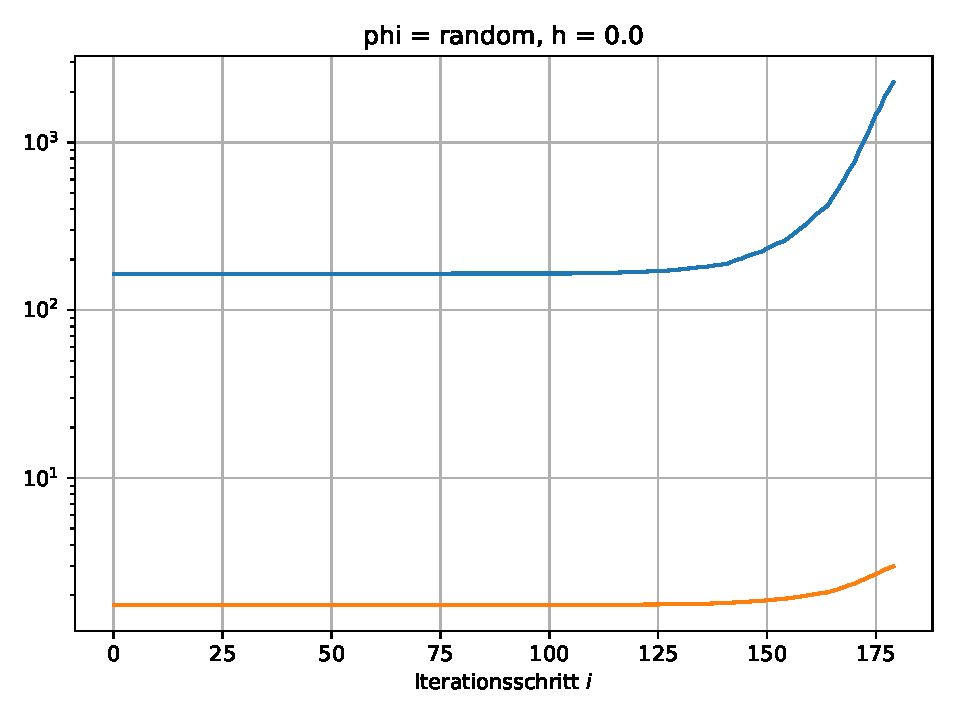
\includegraphics[width=\textwidth]{../figures/phi_rand_h_nil.pdf}
  \caption{Blau: Boltzmann-Exponent, Gelb: Magnetisierung. Zufällige Startkonfiguration, kein äußeres Magnetfeld.}
\end{figure}

\begin{figure}[H]
  \centering
  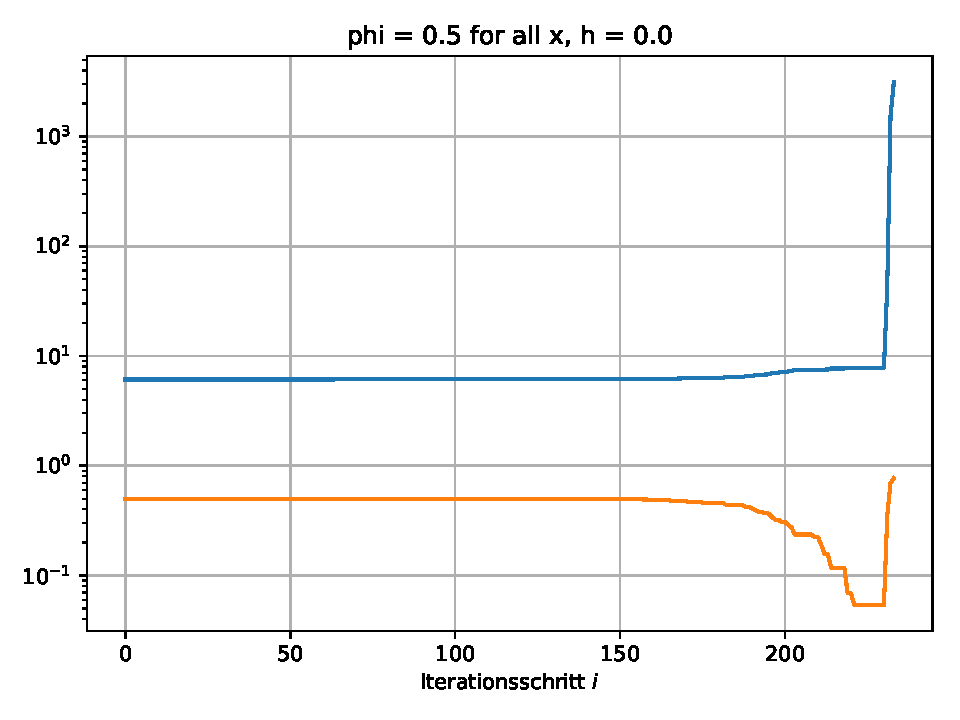
\includegraphics[width=\textwidth]{../figures/phi_pt5_h_nil.pdf}
  \caption{Blau: Boltzmann-Exponent, Gelb: Magnetisierung. Phi konstant, $z=0.5$, kein äußeres Magnetfeld.}
\end{figure}

\begin{figure}[H]
  \centering
  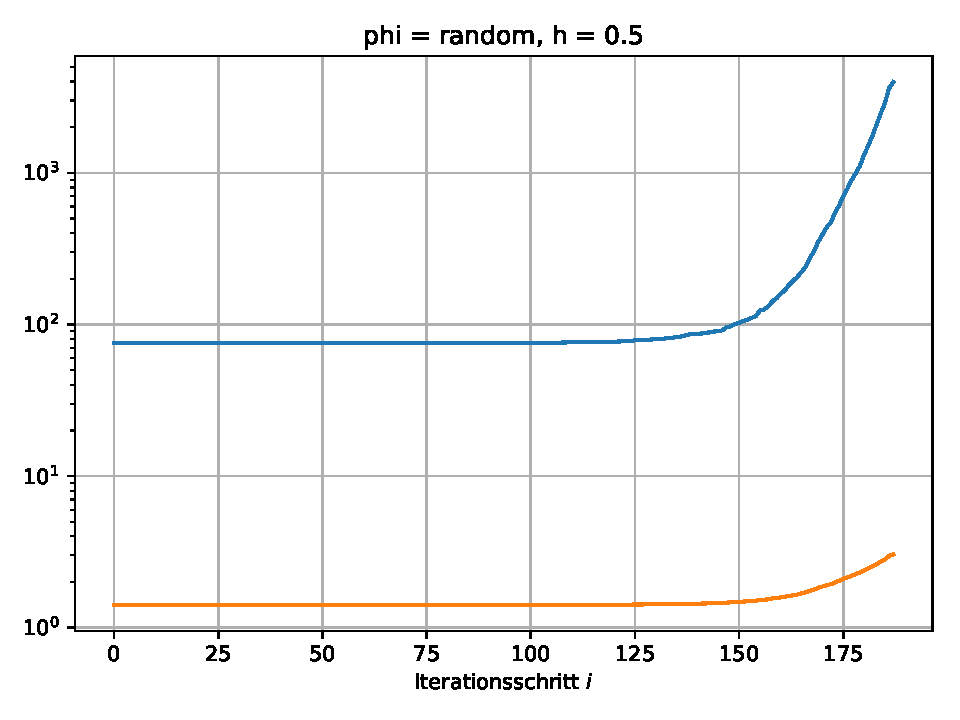
\includegraphics[width=\textwidth]{../figures/phi_rand_h_pt5.pdf}
  \caption{Blau: Boltzmann-Exponent, Gelb: Magnetisierung. Zufällige Startkonfiguration, äußeres Magnetfeld $h=0.5$.}
\end{figure}

\begin{figure}[H]
  \centering
  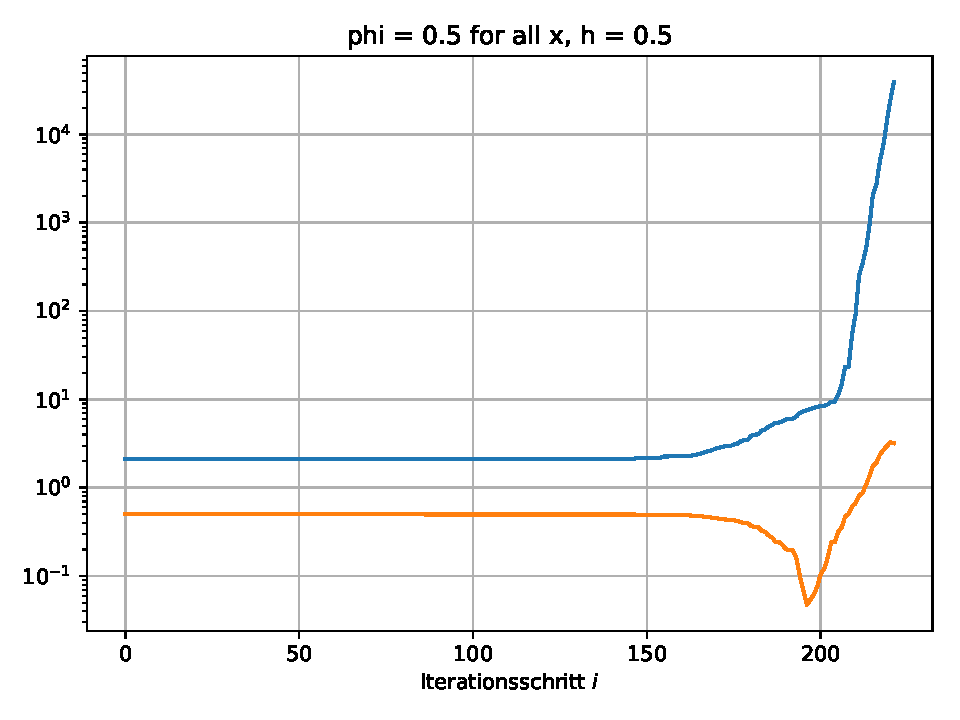
\includegraphics[width=\textwidth]{../figures/phi_pt5_h_pt5.pdf}
  \caption{Blau: Boltzmann-Exponent, Gelb: Magnetisierung. Phi konstant, $z=0.5$, äußeres Magnetfeld $h=0.5$.}
\end{figure}



\end{document}
